\section{Integral calculus}

Calculating discrete sums is rather easy arithmetic, but how about infinite sums? Is it possible to, say, compute the area under a given curve?

\begin{figure}[H]
    \centering

    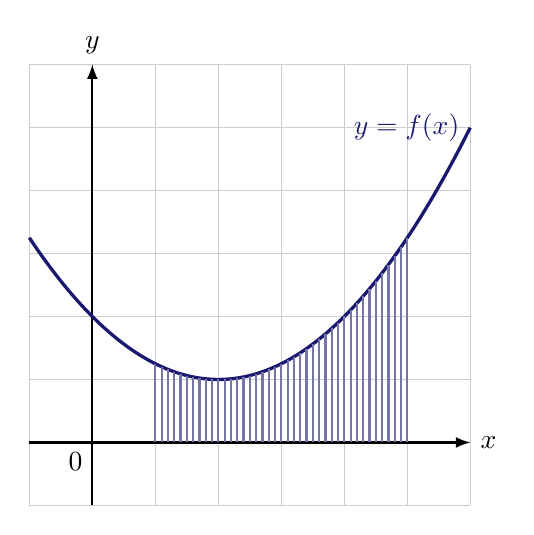
\begin{tikzpicture}[scale=0.8]
        \draw[thin,gray!40] (-1,-1) grid (6, 6);
        \draw[thick, ->, >=latex] (-1,0)--(6,0) node[right]{\(x\)};
        \draw[thick, ->, >=latex] (0,-1)--(0,6) node[above]{\(y\)};
        \draw (0, 0) node[below left] {0};

        \draw [MidnightBlue, very thick, domain=-1:6, samples=100] plot (\x,{0.25*(\x-2)^2+1}) node[left, MidnightBlue] {\(y = f(x)\)};

        \foreach \x in {1,1.1,...,5.1} {
            \draw[MidnightBlue!60, thick] (\x, 0) -- (\x, {0.25*(\x-2)^2+1});
        }

    \end{tikzpicture}
    
    \caption{The area under a quadratic curve.}
    \label{fig:Ch07-area-under-quadratic-curve}
\end{figure}




Let us consider a simpler example, where the curve in question is merely a straight line. Suppose we have a linear function \(f(x) = 2x\). How can we calculate the area under its graph, evaluated between \(x = 0\) and some \(x = a\)?



\begin{figure}[H]
    \centering

    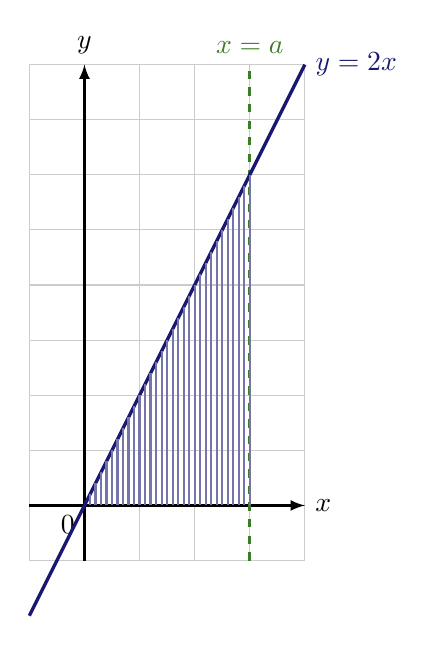
\begin{tikzpicture}[scale=0.7]
        \draw[thin,gray!40] (-1,-1) grid (4, 8);
        \draw[thick, ->, >=latex] (-1,0)--(4,0) node[right]{\(x\)};
        \draw[thick, ->, >=latex] (0,-1)--(0,8) node[above]{\(y\)};
        \draw (0, 0) node[below left] {0};

        \draw[OliveGreen, dashed, very thick] (3, -1) -- (3, 8) node[above] {\(x = a\)};

        \draw [MidnightBlue, very thick, domain=-1:4, samples=100] plot (\x,{2*\x}) node[right, MidnightBlue] {\(y = 2x\)};

        \foreach \x in {0,0.1,...,3.1} {
            \draw[MidnightBlue!60, thick] (\x, 0) -- (\x, {2*\x});
        }
    \end{tikzpicture}
    
    \caption{The area under the straight line given by the function \(y = 2x\).}
    \label{fig:Ch07-area-under-line}
\end{figure}



Geometry tells us that the area of this triangle can be calculated as
%
\[\frac{1}{2} (a)(2a) = a^2\text{.}\]
%
If we rename our variable \(a\) as \(x\), we see that the area under the straight line \(y = 2x\) evaluated between \(0\) and some real number \(x\) can be expressed as \(x^2\). Notice that differentiating \(x^2\) gives us \(2x\), which is our original linear function!

This is by no means a coincidence --- in fact, the process of finding the area under a curve is the inverse operation of differentiation. This process of finding a primitive or antiderivative of a function is known as \textit{integration}, which will be the focus of this section.




\subsection{What is an indefinite integral?}

Recall from the previous section that if \(f\) is the derivative of \(F\), then \(F\) is called a \textit{primitive} or \textit{antiderivative} of \(f\). For example, \(x^2\) is a primitive of \(2x\).
%
\[x^2 \;\;{\color{BrickRed}\rightleftarrows}\;\; 2x\]
%
However, that this is not the only primitive of \(2x\). For instance, \(x^2 + 5\) and \(x^2 - 3\) are both valid antiderivatives. In fact, as we shall prove below, all primitives of \(f\) differ by a constant.

\begin{quote}
    \textbf{Theorem.} for any function \(f\), all primitives of \(f\) differ by a constant.

    \textbf{Proof.} Let \(F_1\) and \(F_2\) be two primitives of \(f\). We want to prove that \(F_1 - F_2\) is a constant.

    To do this, we consider the derivative of the expression \(F_1 - F_2\).
    %
    \begin{align*}
        (F_1 - F_2)' &= F_1' - F_2' \\
        &= f - f\\
        &= 0\text{.}
    \end{align*}
    %
    Since \((F_1 - F_2)' = 0\), the difference \(F_1 - F_2\) must be a constant.
\end{quote}

From this theorem, we conclude that \(x^2 + C\) is a primitive of \(2x\) for any constant \(C\). We can express this fact using an \textit{indefinite integral}, as shown below.
%
\[\int 2x \,dx = x^2 + C\]
%
Here, the constant \(C\) is called the \textit{constant of integration}\footnote{Or: the \textit{integration constant}.}.



\subsection{Rules of integration}

We can modify our rules of differentiation from the last section into rules of integration, some of which are shown below.
%
\newcommand{\redintarrow}{{\;\;\color{BrickRed}\xrightarrow{\int}\;\;}}
%
\begin{align}
    c &\redintarrow cx + C\\
    x &\redintarrow \frac{1}{2}x^2 + C\\
    x^p &\redintarrow \frac{1}{p+1} x^{p+1} + C\\
    e^x &\redintarrow \frac{1}{p+1} e^x + C\\
    \frac{1}{x} &\redintarrow \ln{\abs{x}} + C\\
    \sin{x} &\redintarrow -\cos{x} + C\\
    \cos{x} &\redintarrow \sin{x} + C
\end{align}
%
Here, \(c\) is a constant, \(p\) is a real number, and \(C\) is the constant of integration\footnote{The rules for integration are essentially the reverse of the rules for differentiation, with a few exceptions. For example, the integral of \(1/x\) is \(\ln{\abs{x}}\) rather than \(\ln{x}\), as the natural logarithm is only defined for positive numbers.}. We've left out the product rule and chain rule for now, but we'll see how they can be applied to integration later on.



\subsection{Integration by substitution}

\textit{Integration by substitution} is a powerful technique for integrating functions that are not immediately obvious. Consider, for example, the integral below.
%
\[\int 2x \sqrt{x^2+1} \,dx\]
%
This integral is seems a little tricky at first glance, but we can make it easier by substituting \(u = x^2 + 1\). This substitution gives us
%
\[\frac{du}{dx} = 2x\text{.}\]
%
Not so rigorously, we can rearrange this equation to obtain
%
\[du = 2x\,dx\]
%
the right-hand-side of which is part of our original integral. We can now rewrite our integral in terms of \(u\) like so:
%
\begin{align*}
    \int 2x \sqrt{x^2+1} \,dx &= \int \sqrt{u} \,du\\
    &= \int u^{\frac{1}{2}} \,du\\
    &= \frac{2}{3} u^{\frac{3}{2}} + C\\
    &= \frac{2}{3} (x^2 + 1)^{\frac{3}{2}} + C
\end{align*}
%
which gives us the answer.

Upon closer examination, one can find that integration by substitution is but the chain rule in disguise, as shown below.
%
\begin{align*}
    \frac{d}{dx} f(g(x)) &= f'(g(x)) \cdot g'(x) \tag{chain rule}\\
    \int \frac{d}{dx} f(g(x)) \, dx &= \int f'(g(x)) \cdot g'(x) \,dx \tag{integrate both sides}\\
    f(g(x)) + C &= \int f'(g(x)) \cdot g'(x) \,dx \tag{integral and derivative cancel out}\\
    \int f'(g(x)) \cdot g'(x) \,dx &= f(g(x)) + C \tag{integration by substitution}
\end{align*}



\subsection{Integration by parts}

Another useful technique for integration is \textit{integration by parts}. As an example, consider the following integral.
%
\[\int x \cos{x} \,dx\]

We know that
%
\[\frac{d}{dx} \sin{x} = \cos{x}\]
%
which again after some not-so-rigorous rearrangement gives us
%
\[d(\sin{x}) = \cos{x}\,dx\text{.}\]
%
This allows us to transform our original integral into
%
\[\int x \cos{x} \,dx = \int x \,d(\sin{x})\]
%
but now we're stuck.

Fortunately, integration by parts tells us that whenever we have an integral of the form
%
\[\int f(x) \,d(g(x))\]
%
we can rewrite it as
%
\begin{align*}
    &\; f(x) \cdot g(x) - \int g(x) \,d(f(x))\\
    =&\; f(x) \cdot g(x) - \int g(x) f'(x) \,dx\text{.}
\end{align*}

Hence, we can continue our calculation as follows.
%
\begin{align*}
    \int {\color{BrickRed}x} \,d({\color{MidnightBlue} \sin{x}}) &= {\color{BrickRed}x} \cdot {\color{MidnightBlue} \sin{x}} - \int {\color{MidnightBlue} \sin{x}} \,d({\color{BrickRed}x})\\
    &= {\color{BrickRed}x} \cdot {\color{MidnightBlue} \sin{x}} - \int {\color{MidnightBlue} \sin{x}} \,d{\color{BrickRed}x}\\
    &= x \sin{x} + \cos{x} + C
\end{align*}


\subsection{What is a definite integral?}

